\subsection{Analog-to-Digital Converter} \label{sec:ADC_imp}
Mikrokontrolleren, der avendes som løsningsstrategi i \autoref{sec:loesningsstrategi}, har en Sucessive Approximation Register (SAR) ADC, som gør det muligt at konvertere det analoge signal til et digitalt. Der ønskes en konfigurering af 3 analoge kanaler, herunder Y-aksen på begge accelerometre samt output fra EMG-forstærkeren. Opsætningen af ADC'en på mikrokontrolleren fremgår af \autoref{fig:ADC_teori}. Da ingen af input-signalerne er differentielt opsættes ADC'en til at måle single ended. Hvorfor hvert negativt input for kanalerne er tilkoblet $V_{ss}$, der fungerer som jord. Da der ligeledes ønskes at anvende en 12 bits-ADC på baggrund af kravet i \autoref{sec:ADC_teori}, indstilles denne til en opløsning på 12 bit. Da der anvendes en single ended konfiguration af kanalerne, svarer dette til, at ADC'en kun anvender 11 bit. ADC'ens arbejdsområde er defineret til $3,3~V$, hvoraf  LSB'en for ADC'en kan beregnes ud fra \autoref{equ:LSB}, hvilket giver $2,44~mV$. Hvis der sker ændringer i signalet, der er mindre end LSB på $2,44~mV$, vil dette ikke komme til udtryk i det konverterede signal. 


\begin{figure}[H]
\centering
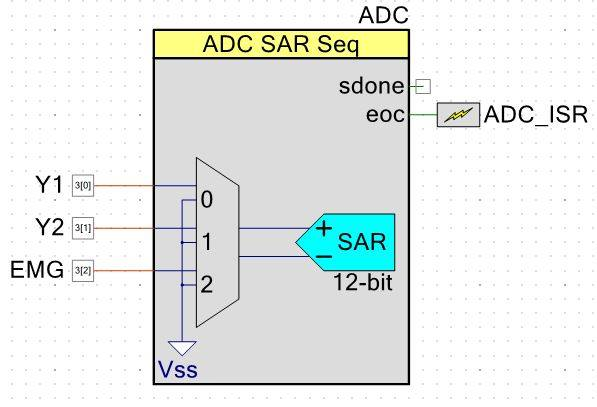
\includegraphics[width=0.5\textwidth]{figures/implementering/ADC_imp.jpg}
\caption{ADC'ens opsætning på PSoC. SAR er ADC typen. Kanalerne Y1, Y2 og EMG er de kanaler, der modtager signaler fra henholdsvis accelerometret, der er placeret på femur, accelerometret, der er placeret på tibia, og EMG-signal. sdone er en outputterminal, der signalerer, at ADC'en har samplet det aktuelle input. End of conversion (eoc) signalerer, når en konversionscyklus er gennemført, dermed kan værdierne fra de samplede kanaler aflæses i samplingsregistret. Når eoc signalerer dette laver ADC'ens Interrupt Service Routine (ISR), som fremgår som ADC\_ISR, et interrupt, hvor værdierne for samplingsregisterer aflæses i nye variabler \citep{ADC2014}.}
\label{fig:ADC_teori}
\end{figure}

\noindent
I ADC'en er der indbygget en clock frekvens. Det er muligt at reducere konverteringstiden ved at øge ADC'ens clock frekvens, der kan indstilles mellem $1000~MHz$ og $9000~MHz$ \citep{ADC2014}. Indstillingen for ADC'en fremgår af \autoref{sec:ADC_bilag}- Clock cycles betegner tiden mellem to efterfølgende impulser fra en oscillator, og samplingtiden måles i clock cycles. Der er forskellige parametre, der kan indstilles i ADC'en, herunder opløsning, samplingsrate og clock frekvens. Disse parametre bestemmer ADC'ens konverteringsrate. %Konvertingstiden er den inverse af konverteringsraten. 

Da der ønskes at sample med 10 gange det opsamlede signals frekvensområde, hvilket ifølge \autoref{sec:pilotforsoeg} er mellem 0,4 og $10~Hz$, vælges der at sample med $100~Hz$. 
I det der defineres en samplingsfrekvens på $100~Hz$ oplyser ADC'en en aktuel samplingsfrekvens per kanal og aktuel clock frekvens. Den aktuelle samplefrekvens oplyses til $97~Hz$. Til at opnå den ønskede frekvens ændres i clock cycles, der ændrer tiden for konverteringstiden for hver kanal. Dette ændres så en konverteringstid $3,32~ms$ opnås. Hertil oplyses den aktuelle samplingsfrekvens som værende $100~Hz$ samt en clock frekvens på $1600~kHz$. 
Som det fremgår af \autoref{fig:ADC_teori}, er outputtet fra ADC'en tilkoblet via eoc til ISR. Hvis der er sker et interrupt vil dette resultere i, at registerene er klar til at blive læst\citep{ADC2014}.


